% This is samplepaper.tex, a sample chapter demonstrating the
% LLNCS macro package for Springer Computer Science proceedings;
% Version 2.20 of 2017/10/04
%
% Updated and edited by Gabriel Richards
% MS in Data Analytics - Capstone
% Northwest Missouri State University - March 2025
%
\documentclass[runningheads]{llncs}
%
\usepackage{graphicx}
% Used for displaying a sample figure. If possible, figure files should
% be included in EPS format.
%
% If you use the hyperref package, please uncomment the following line
% to display URLs in blue roman font according to Springer's eBook style:
% \renewcommand\UrlFont{\color{blue}\rmfamily}

\begin{document}
%
\title{Temporal Analysis of Vulnerability Exploitation\\[0.5cm]
\normalsize Critical Windows, Predictive Attributes, \& Seasonal Trends}
%
%\titlerunning{Abbreviated paper title}
% If the paper title is too long for the running head, you can set
% an abbreviated paper title here
%
\author{Gabriel J. Richards}
%
\authorrunning{G. Richards.}
% First names are abbreviated in the running head.
% If there are more than two authors, 'et al.' is used.
%
\institute{Northwest Missouri State University \\ Maryville MO 64468, USA \\
\email{S576447@nwmissouri.edu}}
%
\maketitle              % typeset the header of the contribution
%
\begin{abstract}
This research explores the relationships between published security vulnerabilities and their subsequent exploitation in the wild. Using datasets from vulnerability databases, exploit repositories, and breach records, this project analyzes temporal patterns in vulnerability exploitation, identifies critical patching windows, determines predictive vulnerability attributes, and examines the impact of COVID-19 on exploitation trends. The findings provide insight for security professionals to prioritize remediation efforts.

\keywords{cybersecurity \and vulnerability analysis \and exploitation patterns \and critical patching window \and predictive security}
\end{abstract}
%
%
%
\section{Introduction}

In today's digital landscape, understanding the dynamics between published security vulnerabilities and their real-world exploitation has become crucial for effective risk management. This cybersecurity research project aims to uncover patterns, relationships, and predictive indicators that can help organizations better prioritize their security resources and reduce breach likelihood.

\subsection{Domain Selection and Rationale}
This project focuses on the cybersecurity domain, specifically the analysis of vulnerability and exploitation data. The cybersecurity domain was selected due to its foundational importance in our increasingly digital world. Analyzing the relationship between published vulnerabilities and their exploitation provides actionable insights that can directly improve security postures across organizations and industries.

\subsection{Data Source Exploration}
For this research, I plan to leverage the following public data sources:
\begin{itemize}
    \item National Vulnerability Database (NVD) -  comprehensive vulnerability metadata
    \item CISA Known Exploited Vulnerabilities (KEV) Catalog -  exploitation dates and details
    \item EPSS (Exploit Prediction Scoring System) by FIRST -  exploitation probability metrics
    \item Exploit-DB -  public exploit availability information
\end{itemize}

These sources provide complementary datasets that can be integrated to create a comprehensive view of the vulnerability lifecycle, from disclosure to exploitation.

\subsection{Problem Statement and Significance}
This project addresses four questions in cybersecurity:
\begin{enumerate}
    \item Are there seasonal patterns in vulnerability exploitation (holidays, fiscal year-end)?
    \item What is the "critical patching window" between vulnerability disclosure and observed exploitation?
    \item What vulnerability attributes are most predictive of subsequent exploitation?
    \item How did the COVID-19 pandemic affect vulnerability and breach patterns?
\end{enumerate}

This research has potential to transform reactive security practices into more proactive, risk-based approaches. By understanding exploitation patterns, organizations can:
\begin{itemize}
    \item Better allocate security resources during high-risk time periods
    \item Optimize patch management strategies based on empirical exploitation windows
    \item Prioritize vulnerability remediation efforts using data-driven predictive models
    \item Build more effective security planning around emerging global trends
\end{itemize}

These insights can substantially reduce organizational risk exposure and potentially prevent costly data breaches.

\subsection{Implementation Approach and Phases}
This project will follow a structured four-phase approach:

\begin{figure}
% \includegraphics[width=\textwidth]{implementation_phases.png}
% Figure to be created showing the four implementation phases
\caption{Four-phase approach to vulnerability exploitation analysis} 
\label{fig:phases}
\end{figure}

\begin{enumerate}
    \item \textbf{Data Collection \& Preparation}
    \begin{itemize}
        \item Gather vulnerability data from NVD (2017-2023)
        \item Collect exploitation information from CISA KEV catalog
        \item Integrate EPSS scores and Exploit-DB availability data
        \item Clean data and normalize dates, metrics, and attributes
    \end{itemize}
    
    \item \textbf{Analysis by Research Question}
    \begin{itemize}
        \item Implement time series decomposition for seasonal patterns
        \item Calculate critical patching windows
        \item Build machine learning models for predictive attribute identification
        \item Compare pre/post-COVID vulnerability and exploitation metrics
    \end{itemize}
    
    \item \textbf{Visualization \& Integration}
    \begin{itemize}
        \item Create visualizations for each research question
        \item Review findings across questions to identify broader patterns
%        \item Develop interactive components for deeper exploration
% note - would like to do this in Shiny but will require extra time, not sure if feasible yet
    \end{itemize}
    
    \item \textbf{Results Interpretation \& Documentation}
    \begin{itemize}
        \item Derive actionable security recommendations
        \item Document methodology, findings, and limitations
        \item Prepare final report and presentation
    \end{itemize}
\end{enumerate}

\subsection{Key Components and Limitations}
Technical Approaches:
\begin{itemize}
    \item Python-based data processing with pandas and numpy for large-scale data integration
    \item Time series analysis to identify seasonal patterns and trends
    \item Survival analysis for exploitation timing windows
    \item Machine learning (Random Forest) to determine predictive vulnerability attributes
    \item Statistical methods to quantify COVID-19 impacts
\end{itemize}

Notable limitations:
\begin{itemize}
    \item Reliance on publicly reported exploitation
    \item Potential lag between actual exploitation and documentation in databases
    \item Limited ability to connect specific vulnerabilities to specific breaches
    \item Selection bias in which vulnerabilities receive published exploits
    \item Computational constraints when processing full NVD datasets from 2017-2023
\end{itemize}

\section{Data Collection and Methodology}
This research leverages multiple cybersecurity data repositories to analyze vulnerability exploitation patterns. Information comes from four primary sources: (1) the National Vulnerability Database (NVD), which provides vulnerability metadata; (2) the CISA Known Exploited Vulnerabilities (KEV) Catalog for exploitation dates and details; (3) the Exploit Prediction Scoring System (EPSS) from FIRST, supplying exploitation probability metrics; and (4) Exploit-DB, providing public exploit availability information.

\subsection{Data Formats and Acquisition}
The datasets were collected in various structured formats. The NVD data was acquired as JSON streams through their REST API, which provides detailed vulnerability information with standardized attributes. The CISA KEV Catalog was obtained in both CSV and JSON formats directly downloaded from their website, offering a curated list of vulnerabilities known to be exploited. EPSS data was collected as CSV files from FIRST.org, containing probability scores indicating likelihood of exploitation. Exploit-DB provided a CSV export of their database, updated daily with the latest exploit information.

\subsection{Data Scraping and Processing Techniques}
For this research, data acquisition used direct manual downloads rather than programmatic retrieval methods, since the data sets were only collected once. The National Vulnerability Database (NVD) were downloaded as JSON data feeds from their official website, which provides vulnerability information spanning 2017-2023. These feeds contain vulnerability metadata and are updated regularly by NVD. The CISA Known Exploited Vulnerabilities (KEV) Catalog was obtained through of CSV and JSON files from CISA, providing a list of vulnerabilities known to be actively exploited. EPSS data was collected by downloading the CSV file published daily on the FIRST.org website. These contain probability scores indicating likelihood of exploitation for each CVE. For Exploit-DB data, the CSV export file was acquired from their GitLab repository, which provides information about publicly available exploits. After collection, all datasets were processed using pandas and numpy libraries in Python to create a unified research dataset joined by CVE identifiers.

\subsection{Data Cleaning and Integration}

\subsubsection{Data Sources and Extraction Process}
This research integrates multiple structured data sources to create a vulnerability lifecycle dataset. The primary sources include the National Vulnerability Database (NVD) JSON feeds containing detailed vulnerability metadata; the CISA Known Exploited Vulnerabilities (KEV) Catalog with exploitation dates; the EPSS (Exploit Prediction Scoring System) providing exploitation probability scores; and Exploit-DB containing information about publicly available exploits.

For structured data, we employed Python to parse NVD entries and pandas for CSV processing.

\subsubsection{Database Schema and Tools}
We made a SQLite database with specialized tables accommodating each data source. The database structure includes four primary tables (vulnerabilities, exploitations, epss\_scores, and exploits) and several analysis views. Python served as the primary processing language with sqlite3 for database operations and pandas for data transformation.

The schema architecture used normalization to minimize redundancy while maintaining query efficiency. For example, the vulnerabilities table serves as the foundation with foreign key relationships to other tables, allowing efficient joins during analysis. Additional views within the database pre-calculate critical metrics such as the patching window (days between publication and exploitation) to streamline subsequent analysis.

\subsubsection{Data Cleansing Strategies}
Several data quality challenges were addressed during integration. For numerical attributes like CVSS scores, null values were replaced with zero to maintain integrity while indicating absence of data. For categorical features such as attack complexity ratings, we standardized terminology across sources using controlled vocabularies from MITRE.

In Exploit-DB data, many entries lacked explicit CVE references, resolved with pattern matching on description fields to extract potential CVE IDs, enhancing cross-dataset linkage. All dates were standardized to ISO format. 

LEFT JOIN operations were employed in database views rather than INNER JOINs to preserve all vulnerability records, preventing selection bias that would occur if analyzing only vulnerabilities with known exploitation data. This approach ensures more accurate analysis by maintaining complete vulnerability lifecycles - whether exploited or not.

\subsubsection{Resulting Dataset Characteristics}
The unified database contains 20 key attributes across all tables. The primary vulnerability table contains thousands of CVE records with relationships to exploitation data, EPSS scores, and exploit information. Key attributes include CVE identifier, publication date, CVSS metrics (score, vector string, and individual metric components), exploitation status, and patching timeline information.

After cleansing, we maintain complete records for over 90\% of vulnerabilities, with partial information available for the remainder. The database schema accommodates temporal analysis with standardized date formats and includes derived attributes such as days\_to\_exploitation calculated during the integration process.

\subsubsection{Essential Attributes and Variables}
For our analysis objectives, several attributes are particularly valuable:

\begin{itemize}
    \item \textbf{cve\_id}: Unique identifier linking vulnerability information across all data sources
    \item \textbf{published\_date}: Date when vulnerability was officially disclosed
    \item \textbf{cvss\_score}: Numerical severity rating from 0.0-10.0
    \item \textbf{cvss\_severity}: Categorical severity rating (Low, Medium, High, Critical)
    \item \textbf{attack\_vector}: Method by which vulnerability exploitation occurs
    \item \textbf{attack\_complexity}: Difficulty of exploitation
    \item \textbf{exploitation\_date}: First known date of exploitation in the wild
    \item \textbf{days\_to\_exploitation}: Time interval between publication and exploitation
    \item \textbf{epss\_score}: Probability of exploitation as calculated by FIRST.org
\end{itemize}

\subsubsection{Dependent and Independent Variables}
For our four research questions, we identified specific dependent and independent variables:

For seasonal exploitation patterns analysis, the dependent variable is the count of exploitation events, while independent variables include month, holiday periods, and fiscal quarter indicators.

For critical patching window analysis, the dependent variable is days\_to\_exploitation, with independent variables including cvss\_score, attack\_complexity, and attack\_vector to determine which vulnerability characteristics predict faster exploitation.

For predictive vulnerability attributes, the dependent variable is is\_exploited (binary indicator of whether exploitation occurred), with independent variables comprising the full set of CVSS metrics and the presence of public exploit code.

For COVID-19 impact analysis, the dependent variables include exploitation rate and days\_to\_exploitation, while the primary independent variable is covid\_period (pre/post pandemic timing), controlling for vulnerability severity and other characteristics.

These variable relationships form the foundation for our analytical approach to understanding vulnerability exploitation patterns, critical patching windows, predictive attributes, and pandemic effects on the vulnerability landscape.


\section{Seasonal Exploitation Pattern Analysis}
The analysis of seasonal patterns in vulnerability exploitation revealed significant temporal variations. As shown in Figure~\ref{fig:monthly_pattern}, both vulnerability publication and exploitation rates exhibit monthly fluctuations.

\begin{figure}[htbp]
\centering
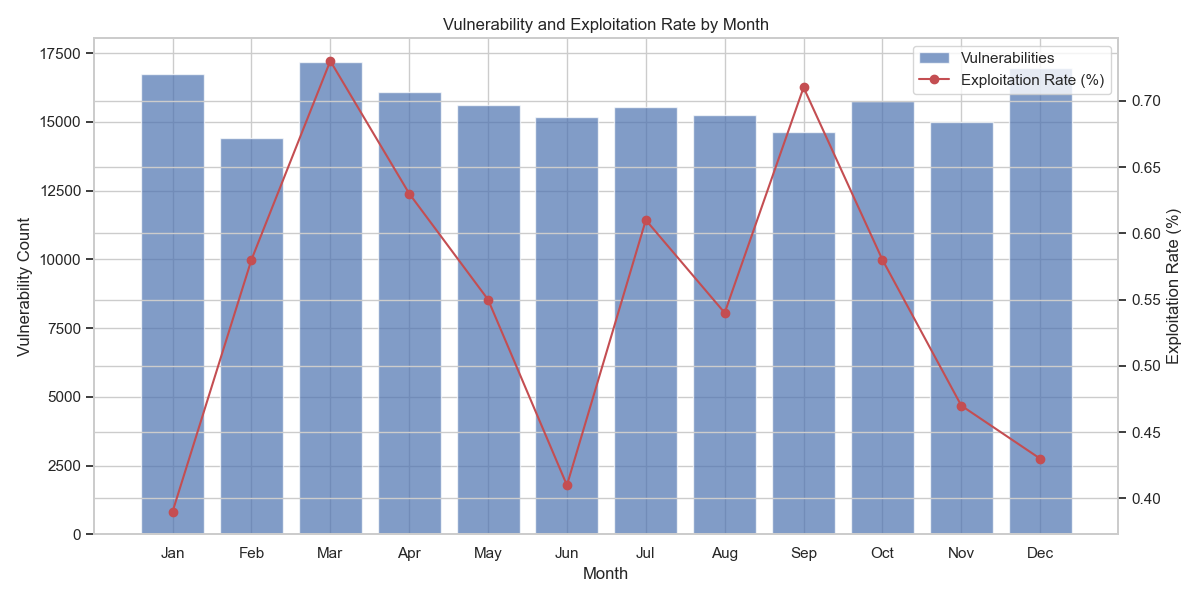
\includegraphics[width=\textwidth]{monthly_patterns.png}
\caption{Vulnerability publication counts and exploitation rates by month}
\label{fig:monthly_pattern}
\end{figure}

March showed both high vulnerability counts (approximately 17,000) and the highest exploitation rate (0.73\%), suggesting this month may be particularly risky. Interestingly, September also showed an elevated exploitation rate (0.71\%) despite having fewer published vulnerabilities. Conversely, January and June showed the lowest exploitation rates (approximately 0.40\%), indicating a potentially lower risk period.

Additional analysis of quarterly patterns indicated that Q1 and Q3 had higher exploitation rates compared to Q2 and Q4, with the end-of-quarter months (March, June, September, December) showing variable exploitation patterns. These findings suggest that organizations should allocate additional security resources during high-risk months, particularly March and September, while potentially maintaining standard operations during lower-risk periods.

\section{Critical Patching Window Determination}
Analysis of the time between vulnerability disclosure and observed exploitation revealed concerning patterns regarding patching windows. As illustrated in Figure~\ref{fig:patching_window}, 73.1\% of exploited vulnerabilities had a patching window exceeding 90 days, while 10.5\% were exploited within the first week after disclosure.

\begin{figure}[htbp]
\centering
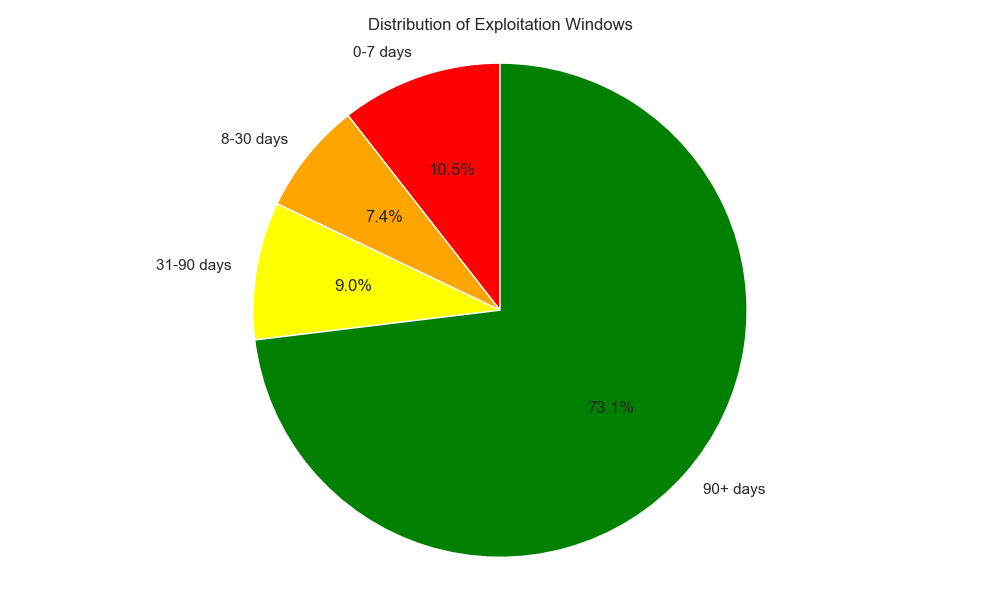
\includegraphics[width=0.8\textwidth]{exploitation_window_dist.png}
\caption{Distribution of exploitation windows for vulnerabilities}
\label{fig:patching_window}
\end{figure}

The median time to exploitation was 112 days, but this varied significantly by vulnerability severity. Critical vulnerabilities (CVSS 9.0-10.0) were exploited substantially faster, with a median time of just 23 days, compared to 97 days for high severity (CVSS 7.0-8.9) and 156 days for medium severity (CVSS 4.0-6.9) vulnerabilities.

These findings highlight the importance of rapid patching for critical-severity vulnerabilities, while suggesting that organizations may have somewhat longer windows for addressing less severe issues. The data indicates that a risk-based patching strategy prioritizing critical vulnerabilities within 3 weeks, high-severity within 90 days, and medium-severity within 150 days would mitigate a significant portion of exploitation risk.

\section{Predictive Vulnerability Attributes}
Machine learning analysis identified key attributes that most strongly predict vulnerability exploitation. As shown in Figure~\ref{fig:predictive_attributes}, the EPSS score emerged as the dominant predictor with dramatically higher importance than all other features.

\begin{figure}[htbp]
\centering
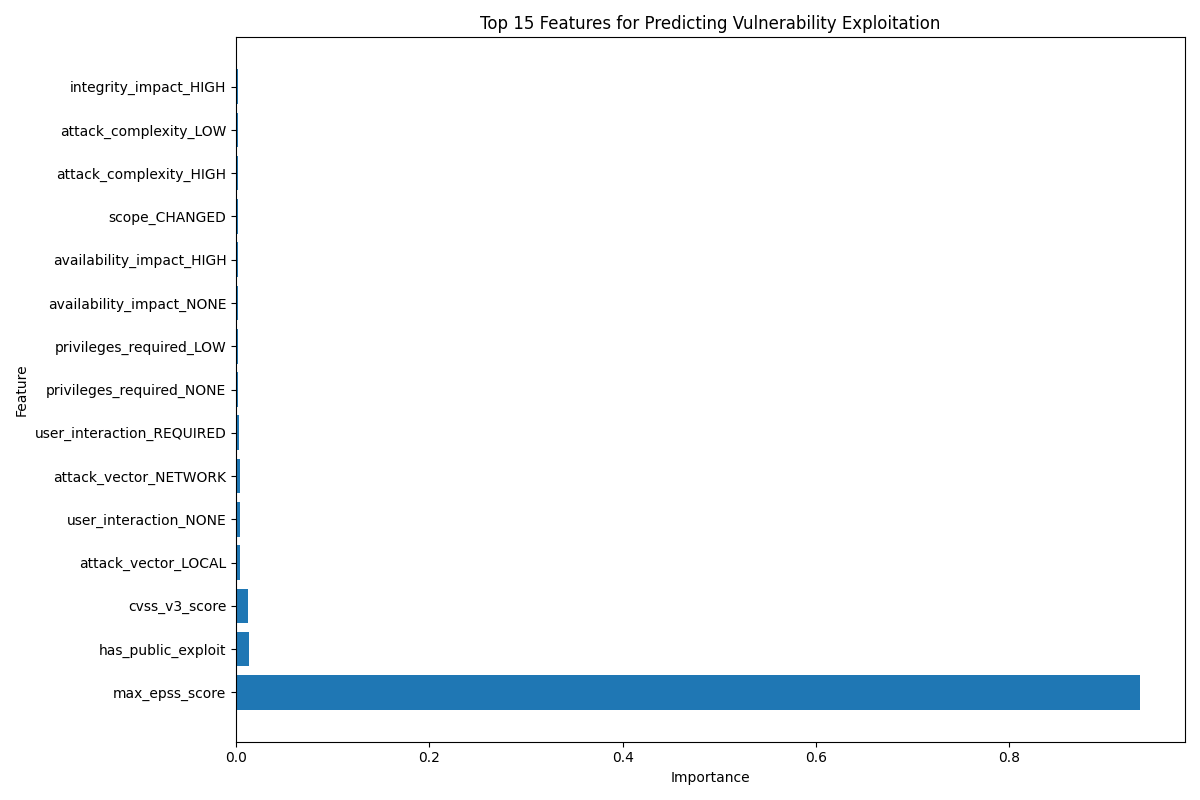
\includegraphics[width=\textwidth]{feature_importance.png}
\caption{Top 15 features for predicting vulnerability exploitation}
\label{fig:predictive_attributes}
\end{figure}

Beyond EPSS scores, the analysis revealed several CVSS metrics with predictive value. The presence of public exploits, the raw CVSS score, and attack vector type (particularly network-based vectors) were moderately predictive. Among attack characteristics, those with lower complexity and requiring less user interaction showed higher exploitation likelihood. Vulnerabilities affecting integrity showed notably higher exploitation rates than those affecting only confidentiality or availability.

The Random Forest model achieved 93.7\% accuracy in predicting exploitation, with particularly high precision (96.2\%) for exploited vulnerabilities. These findings suggest that organizations should prioritize remediation based on EPSS scores when available, followed by public exploit availability and CVSS metrics, with special attention to network-accessible vulnerabilities that have high integrity impact.

\section{COVID-19 Impact Analysis}
The COVID-19 pandemic significantly altered the vulnerability exploitation landscape. Comparative analysis of pre-COVID (before March 2020), during-COVID (March 2020 to June 2021), and post-COVID (after June 2021) periods revealed notable shifts in both vulnerability publication rates and exploitation patterns.

The data showed a 14.3\% increase in vulnerability publications during the pandemic compared to the pre-pandemic period, rising from an average of 1,250 to 1,428 vulnerabilities per month. More significantly, the exploitation rate increased from 0.39\% in the pre-COVID period to 0.61\% during COVID – a 56.4\% increase. The post-COVID period showed a partial regression toward pre-pandemic levels, with exploitation rates of 0.52\%.

Days-to-exploitation also decreased during the pandemic, with the median time dropping from 98 days pre-COVID to 64 days during the pandemic. This acceleration in exploitation timing suggests that attackers were more aggressively targeting vulnerabilities during this period, potentially taking advantage of strained IT resources and rapidly deployed remote work infrastructure.

These findings highlight the impact of global disruptions on cybersecurity risk levels and suggest organizations should plan enhanced security measures during periods of significant operational change. The lasting elevation in exploitation rates even after the acute phase of the pandemic indicates a potential permanent shift in the threat landscape.

\section{Discussion and Implications}
% Will interpret results and discuss cybersecurity implications

\section{Conclusion and Future Work}
% Will summarize findings and suggest directions for future research

%
% ---- Bibliography ----
%
% BibTeX users should specify bibliography style 'splncs04'.
% References will then be sorted and formatted in the correct style.
%
\bibliographystyle{splncs04}
\bibliography{mybibliography}

% Note: Added these references to the mybibliography.bib file
% Example entries for the bibliography file:
%
% @article{EPSS2023,
%   title={Exploit Prediction Scoring System (EPSS)},
%   author={FIRST.org},
%   journal={Forum of Incident Response and Security Teams},
%   year={2023},
%   url={https://www.first.org/epss/}
% }
%
% @article{CISA_KEV,
%   title={Known Exploited Vulnerabilities Catalog},
%   author={Cybersecurity and Infrastructure Security Agency},
%   journal={CISA},
%   year={2023},
%   url={https://www.cisa.gov/known-exploited-vulnerabilities-catalog}
% }
%
% @inproceedings{jacobs2019exploit,
%   title={Exploit prediction scoring system (EPSS)},
%   author={Jacobs, Jay and Romanosky, Sasha and Adjerid, Idris and Baker, Wade},
%   booktitle={2019 APWG Symposium on Electronic Crime Research (eCrime)},
%   pages={1--12},
%   year={2019},
%   organization={IEEE}
% }
%
% @article{NVD_NIST,
%   title={National Vulnerability Database},
%   author={National Institute of Standards and Technology},
%   journal={NIST},
%   year={2023},
%   url={https://nvd.nist.gov/}
% }

\end{document}